\chapter{Feasibility}
This system needs requirements listed below:
\begin{itemize}
    \item This system needs real time location of user. So this system needs to run on mobile devices.
    \item This system must provide interaction within users. So to provide intraction of multiple mobile devices this system needs to a server side.
    \item In process of development to provide version controlling Git must used as VCS.
\end{itemize}

\section{Technic Feasibility}
\subsection{Software Feasibility}
In this section there are descriptions about choosing database system, web server system, development language and development enviroment.
As a result of feasibility workings we decided to do server side programming with Java programming language. Because of two of developers working of this project knows Java well, Java is object oriented language, Android can be programming with Java natively, sources about Java can be found easily and Java can run both Android and server.
We don't choosen any cross platform tools for mobile development. Because mobile application must require low power consuption, so that development must be native.
Mobile application will be written for only Android because of anyone in our team doesn't have a MacBook to develop for iOS.

\subsection{Hardware Feasibility}
For a small number of users like 1 to 100 it is enough to use 1 GB ram and 100 GB disk. But for astronomical number of users there must be a cloud storage and powerful servers. For a solution for this scaling problem server side of this project will be settin on AWS.


For the requirements mentioned above the computer which the project is to be developed should be at a level that meets the minimum system requirements mentioned below separeted by mobile and server side.

For Server Side Development:
\begin{itemize}
    \item JDK 1.8
    \item Spring Tool Suit, Spring Boot
    \item Eclipse, Java IDE
    \item Sublime text, gedit etc. text editor
    \item Apache Tomcat or Glassfish
    \item Access key to use Google Maps API
    \item A Browser to render HTML and Javascript
    \item 8 GB RAM minimum, 16 GB RAM recommended
    \item Minimum 250GB Free Disk Space    
    \item Linux or Windows Operating System.
    \item Git
    
\end{itemize}

For Mobile Application Development:
\begin{itemize}
    \item JDK 1.8
    \item Android Studio
    \item Android SDK
    \item Android Emulator
    \item Android System Images
    \item Access key to use Google Maps API
    \item 8 GB RAM and 8 GB swap area minimum, 16 GB RAM recommended
    \item Minimum 250GB Free Disk Space
    \item Linux or Windows Operating System.
    \item Git    
\end{itemize}


\section{Labor Force Feasibility}
There are two people needed for developing mobile and server side of system concurrently.



\section{Time Feasibility}
Gannt diagram shown below.
\begin{figure}[!htbp]
\centering
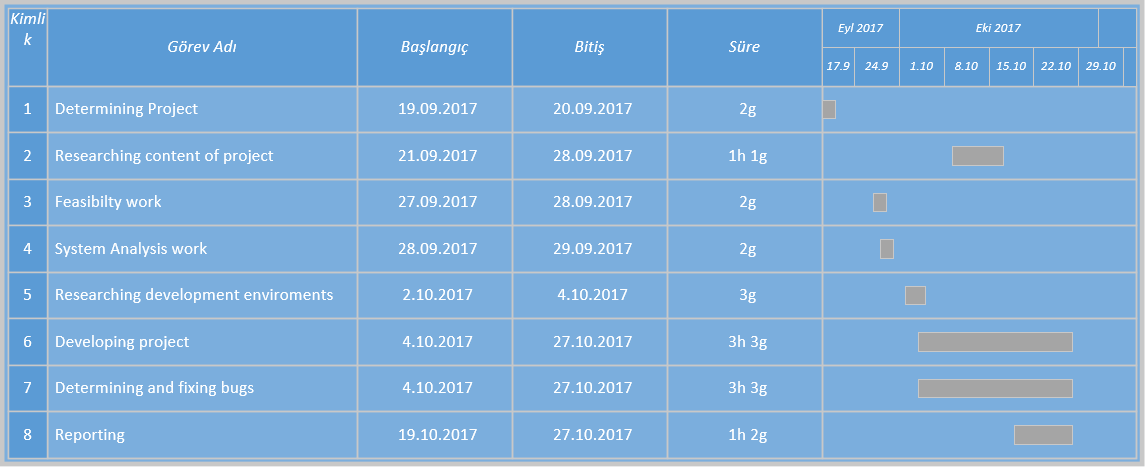
\includegraphics[width=\textwidth]{projectChapters/images/gantt.png}
\caption{Gantt Diyagramı Zaman Çizelgesi}
\end{figure}


\section{Legitimate Feasibility}
There are no patent infringements as the software components to be used in the development phase of the project are open source and free of charge. Users are responsible for the legal problems that may arise due to the shares they have made according to Article 8 of Law No. 5651 and Article 125 of the Turkish Penal Code.


\section{Economic Feasibility}
There is no charge for software components to be used during application development. The hourly working fee of the person who will develop the project is 25 TL per person. The total cost determined for the project during the project development period stated in the Gantt Chart is 8000 TL. The price of a computer with minimum system requirements stated in the title of hardware feasibility which costs currently between 1500 and 2500 TL. Price of Google Map API is 4\$ and 15 TL per month. Price of AWS is 15\$ and 60 TL per month.

\begin{table}[]
\centering
\caption{Total Cost Table For Gezi-Yorum}
\label{my-label}
\begin{tabular}{|l|l|}
\hline
\multicolumn{1}{|c|}{\textbf{Cost}} & \multicolumn{1}{c|}{\textbf{TL}} \\ \hline
Hardware                               & 5.000,00 TL                      \\ \hline
Project Team                           & 16.000,00 TL                      \\ \hline
Google Map API                         & 15,00 TL                      \\ \hline
AWS                                 & 60,00 TL                      \\ \hline
\textbf{Toplam}                        & \textbf{21.075,00 TL}            \\ \hline
\end{tabular}
\end{table}




